\let\negmedspace\undefined
\let\negthickspace\undefined
\documentclass[journal,12pt,twocolumn]{IEEEtran}
\usepackage{cite}
\usepackage{amsmath,amssymb,amsfonts,amsthm}
\usepackage{algorithmic}
\usepackage{graphicx}
\usepackage{textcomp}
\usepackage{xcolor}
\usepackage{txfonts}
\usepackage{enumitem}
\usepackage{mathtools}
\usepackage{gensymb}
\usepackage{comment}
\usepackage[breaklinks=true]{hyperref}
\usepackage{tkz-euclide} 
\usepackage{listings}
\usepackage{gvv}                                        
%\def\inputGnumericTable{}                                 
\usepackage[latin1]{inputenc}                                
\usepackage{color}                                            
\usepackage{array}                                            
\usepackage{longtable}                                       
\usepackage{calc}                                             
\usepackage{multirow}                                         
\usepackage{hhline}                                           
\usepackage{ifthen}                                           
\usepackage{lscape}
\usepackage{tabularx}
\usepackage{array}
\usepackage{float}


\newtheorem{theorem}{Theorem}[section]
\newtheorem{problem}{Problem}
\newtheorem{proposition}{Proposition}[section]
\newtheorem{lemma}{Lemma}[section]
\newtheorem{corollary}[theorem]{Corollary}
\newtheorem{example}{Example}[section]
\newtheorem{definition}[problem]{Definition}
\newcommand{\BEQA}{\begin{eqnarray}}
\newcommand{\EEQA}{\end{eqnarray}}
\newcommand{\define}{\stackrel{\triangle}{=}}
\theoremstyle{remark}
\newtheorem{rem}{Remark}
\begin{document}

\bibliographystyle{IEEEtran}
\onecolumn
\vspace{3cm}
\title{Straight lines and Pair of Straight Lines}
\author{Golla Shriram - AI24BTech11010}

\maketitle
%\newpage
%\bigskip

\renewcommand{\thefigure}{\theenumi}
\renewcommand{\thetable}{\theenumi}

\section{E - Subjective Problems}
                                                                           
 \begin{enumerate}[start=4]


\item                    	\hfill{(1979)}
	\begin{enumerate}
             \item     Two vertices of triangle are \brak{5,-1} and \brak{2,-3}.If the orthocentre of triangle is origin, find the coordinates of the thrid point.
	     \item  Find the equation of the line which bisects the obtuse angle between  the lines $x-2y+4=0$ and $4x-3y+2=0$.
         \end{enumerate}

\item A stright line $L$ is perpendicular to the line $5x-y+1$.The area of the triangle formed by $L$ and the coordinate axes is 5 . Find the equation of the line $L$.\hfill{(1980)}

\item The end $A$,$B$ of a straight line segment of constant lenght c slide upon the fixed rectangle $ OX,OY$ respectively.then show that the locus of the foot of perpendicular drawn from $P$ to $AB$ is 
 \begin{align*}  x^\frac{2}{3} + y^\frac{2}{3} = c^\frac{2}{3} \end{align*}

  \item The vertices of a triangle are $\sbrak{ at_1t_2,a\brak{t_1+t_2}},\\ \sbrak{ at_2t_3,a\brak{t_2+t_3}},\sbrak{at_3t_1,a\brak{t_3+t_1}}$. Find the orthocentre of the triangle. \hfill{(1983-3M)}
	  
\item The coordinates of $A,B,C$ are $ \sbrak{6,3} ,\sbrak{3,5} , \sbrak{4,2} $ respectively, and $P$ is any point $(x,y)$.
Show that the ratio of the area of triangles $\Delta PBC$  and $\Delta ABC$ is $\abs{\frac{x+y-2}{7}}$ \hfill{(1983-2M)} 

\item Two equal sides of an isosceles triangle are given by the equations $7x-y+3=0$ and $x+y-3=0$ and its third side passes through the point $\brak{1,-10}$ . Determine the equation of the third side.  \hfill{(1985-3M)}

\item One of the diameters of the circle circumscribing the rectangle $ABCD$ is $4y=x+ 7$. if $A$ and $B$ are the points $\brak{-3,4}$ and $\brak{5,4}$ respectively, the find the area of rectangle .  \hfill{(1985-3M)}


\item Two sides of a rhombus $ABCD$ are parallel to the lines $y=x+2$ and $y=7x+3$ .If the diagonals of the rhombus intersect at the point $\brak{1,2}$ and the vertex $A$ is on the y-axis , find the possible co-ordinates of $A$.     \hfill{(1985-5M)} 

\item Lines $ L_1 \equiv ax+by+c =0 $ and $ L_2 \equiv lx+my+n =0 $ intersect at the point $P$ and make an angle $\theta$ with each other . Find the equation of a line $L$ different from $L_2$ which passes through $P$ and make same angle $\theta$ with $L_1$ . \hfill{(1988-5M)}


\item Let $ABC$ be the triangle $AB=AC$ . If $D$ is the midpoint of $ BC , E$ is the foot of the perpendicular drawn from $D$ to $AC$ and $F$ the mid-point of $DE$ , prove that $AF$ is perpendicular to $BE.$ \hfill{(1989-5M)}

\item Straight lines $3x + 4y =5$ and $ 4x-3y= 15$ intersect at the point $A$ . Points $B$ and $C$ are chosen on these two lines such that $AB=AC$ .Determine the possible equations of the line $BC$ passing through the point $\brak{1,2}$.\hfill{(1990-4M)}

\item A line cuts the x-axis at $A(7,0)$ and the y-axis at $B(0,-5)$. A variable line $PQ$ is drawn perpendicular to $AB$ cutting the x-axis in $P$ and the y-axis in $Q$. If $AQ$ and $BP$ intersect at $R$, find the locus of $R$.  \hfill{(1990-4M)}

\item Find the equation of the line passing through the point $\brak{2,3}$ and making intercept of length 2 units between the lines $ y + 2x = 3 $ and $ y + 2x = 5  $.     \hfill{(1991-4M)}

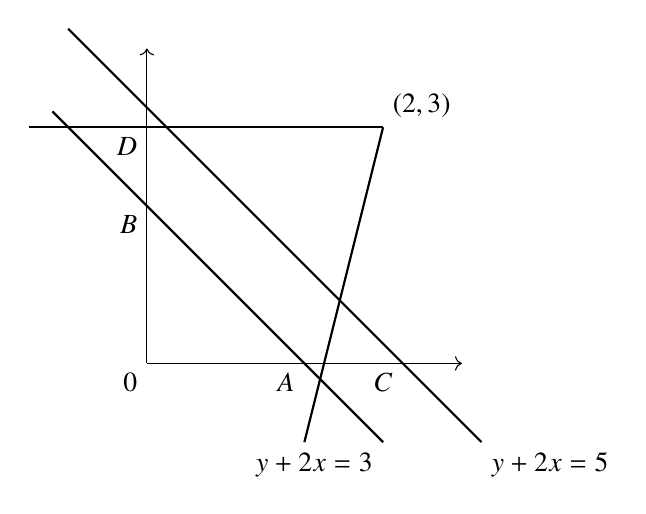
\begin{tikzpicture}
\draw[->] (0,0) -- (4,0) node[right] {};
\draw[->] (0,0) -- (0,4) node[above] {};


\draw[thick] (-1,4.25) -- (4.25,-1) node[below right] {$y + 2x = 5$};
\draw[thick] (-1.2,3.2) -- (3,-1) node[below left] {$y + 2x = 3$};


\filldraw[black] (0,0)  node[below left] {$0$};
\filldraw[black] (2,0)  node[below left] {$A$};
\filldraw[black] (3.25,0)  node[below left] {$C$};
\filldraw[black] (3,3)  node[above right] {$(2,3)$};


\draw[thick] (-1.5,3) -- (3,3) node[midway, right] {};

\draw[thick] (2,-1) -- (3,3) node[midway, right] {};


\node[below left ] at (0,2) {$B$};
\node[below left ] at (-0,3) {$D$};
\end{tikzpicture}



\item Show that all chords of  the curve $ 3x^2-y^2-2x+4y=0,$ which subtend a right angle at the origin.pass through a fixed point . Find the coordinates of point.     \hfill{(1991-4M)}

\item Determine all values of $\alpha$ for which the point ($\alpha , \alpha^2$) lies inside the triangle formed by the lines.  \hfill{(1992-6M)}
	\begin{align*}  2x+3y-1&=0\\ 
	x+2y-3&=0  \\ 5x-6y-1&=0   \end{align*}

\end{enumerate}
\end{document}


